This sentence requires citation \citep{Reference1}. This sentence requires multiple citations to imply that it is better supported \citep{Reference2,Reference3}. Finally, when conducting an appeal to authority, it can be useful to cite a reference in-text, much like \cite{Reference1} do quite a bit. Oh, and make sure to check out the bear in Figure \ref{bear}.

\begin{figure}[h!]
	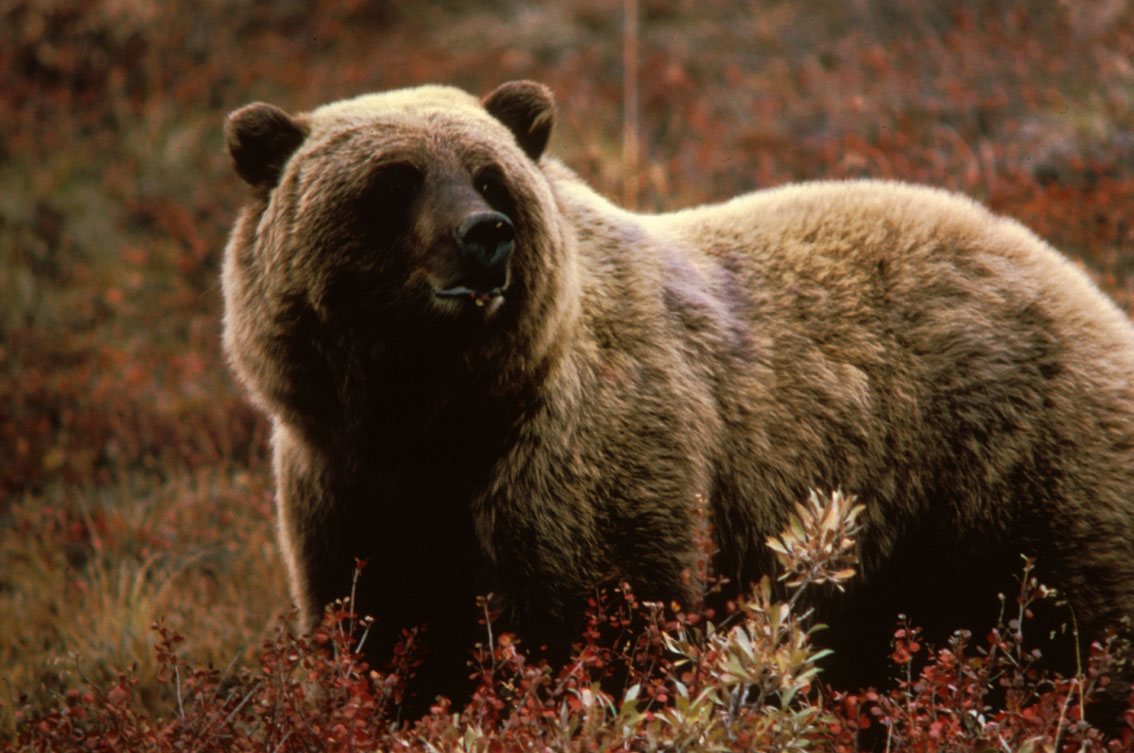
\includegraphics[width=\linewidth]{images/bear.jpg} % Figure image
	\caption{A majestic grizzly bear} % Figure caption
	\label{bear} % Label for referencing with \ref{bear}
\end{figure}

Lorem ipsum dolor sit amet, consectetur adipiscing elit. Fusce maximus nisi ligula. Morbi laoreet ex ligula, vitae lobortis purus mattis vel. Vestibulum ante ipsum primis in faucibus orci luctus et ultrices posuere cubilia Curae; Donec ac metus ut turpis mollis placerat et nec enim. Duis tristique nibh maximus faucibus facilisis. Praesent in consequat leo. Maecenas condimentum ex rhoncus, elementum diam vel, malesuada ante. Fusce pulvinar, mauris pretium placerat venenatis, lectus ex tempus lacus, id suscipit libero lorem eu augue. Interdum et malesuada fames ac ante ipsum primis in faucibus.

\begin{align}
	A = 
	\begin{bmatrix}
		A_{11} & A_{21} \\
		A_{21} & A_{22}
	\end{bmatrix}
\end{align}

Donec nec nibh sagittis, finibus mauris quis, laoreet augue. Maecenas aliquam sem nunc, vel semper urna hendrerit nec. Pellentesque habitant morbi tristique senectus et netus et malesuada fames ac turpis egestas. Maecenas pellentesque dolor lacus, sit amet pretium felis vestibulum finibus. Duis tincidunt sapien faucibus nisi vehicula tincidunt. Donec euismod suscipit ligula a tempor. Aenean a nulla sit amet magna ullamcorper condimentum. Fusce eu velit vitae libero varius condimentum at sed dui.

\begin{itemize}
	\item First item in a list 
	\item Second item in a list 
	\item Third item in a list
\end{itemize}


In non leo tincidunt, tristique orci eu, suscipit ex. Fusce non lectus ut dolor tincidunt fermentum. Donec dictum mauris magna, ut dictum nisl finibus quis. Nulla elementum ipsum ut lectus sodales finibus. Nulla ac malesuada magna. Etiam arcu dolor, luctus eget elit a, volutpat vulputate mi. Donec elementum tellus libero, ut ornare orci dignissim lacinia. Nullam iaculis vehicula sem, at tempor tellus. Praesent eu nisi a elit viverra lobortis. Nullam eu metus et justo molestie posuere vitae imperdiet erat. Praesent at gravida dui. 

\begin{description}
	\item[First] This is the first item
	\item[Last] This is the last item
\end{description}


Donec nec nibh sagittis, finibus mauris quis, laoreet augue. Maecenas aliquam sem nunc, vel semper urna hendrerit nec. Pellentesque habitant morbi tristique senectus et netus et malesuada fames ac turpis egestas. Maecenas pellentesque dolor lacus, sit amet pretium felis vestibulum finibus. Duis tincidunt sapien faucibus nisi vehicula tincidunt. Donec euismod suscipit ligula a tempor. Aenean a nulla sit amet magna ullamcorper condimentum. Fusce eu velit vitae libero varius condimentum at sed dui.

\begin{table}[h!]
	\caption{Example table}
	\centering
	\begin{tabular}{llr}
		\toprule
		\multicolumn{2}{c}{Name} \\
		\cmidrule(r){1-2}
		First Name & Last Name & Grade \\
		\midrule
		John & Doe & $7.5$ \\
		Richard & Miles & $5$ \\
		\bottomrule
	\end{tabular}
\end{table}

Donec nec nibh sagittis, finibus mauris quis, laoreet augue. Maecenas aliquam sem nunc, vel semper urna hendrerit nec. Pellentesque habitant morbi tristique senectus et netus et malesuada fames ac turpis egestas. Maecenas pellentesque dolor lacus, sit amet pretium felis vestibulum finibus. Duis tincidunt sapien faucibus nisi vehicula tincidunt. Donec euismod suscipit ligula a tempor. Aenean a nulla sit amet magna ullamcorper condimentum. Fusce eu velit vitae libero varius condimentum at sed dui.